\documentclass[tikz,border=3.14mm]{standalone}
\begin{document}
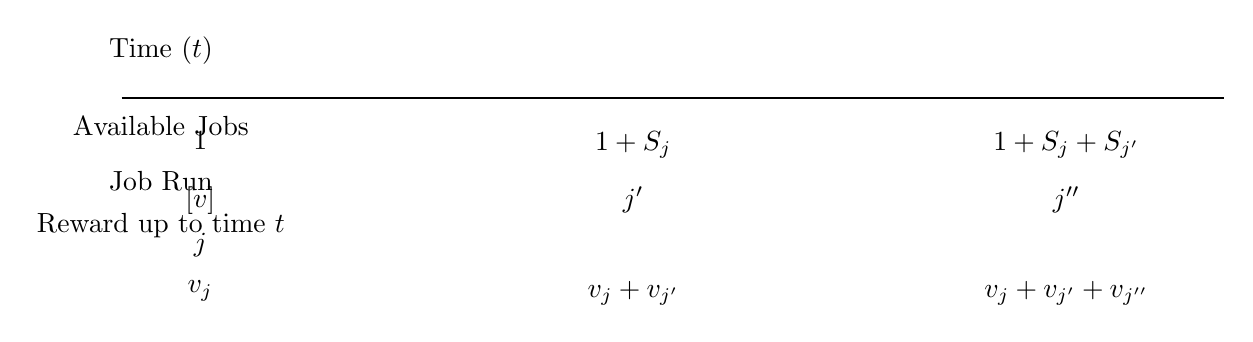
\begin{tikzpicture}[>=latex]
    % Draw the timeline
    \draw (0,0) -- (14,0);
    
    % Time labels
    \draw (0.5,0.3) node[above] {Time ($t$)};
    \draw (1,-0.3) node[below] {$1$};
    \draw (1+5.5,-0.3) node[below] {$1+S_j$};
    \draw (1+5.5+5.5,-0.3) node[below] {$1+S_j+S_{j'}$};
    
    % Available Jobs
    \draw (0.5,-0.6) node[above] {Available Jobs};
    \draw (1,-1) node[below] {$[v]$};
    \draw (1+5.5,-1) node[below] {$j'$};
    \draw (1+5.5+5.5,-1) node[below] {$j''$};
    
    % Job Run
    \draw (0.5,-1.3) node[above] {Job Run};
    \draw (1,-1.6) node[below] {$j$};
    
    % Reward up to time t
    \draw (0.5,-1.9) node[above] {Reward up to time $t$};
    \draw (1,-2.2) node[below] {$v_j$};
    \draw (1+5.5,-2.2) node[below] {$v_j+v_{j'}$};
    \draw (1+5.5+5.5,-2.2) node[below] {$v_j+v_{j'}+v_{j''}$};
    
    % Busy periods (optional, if you want to indicate the busy periods visually)
    % Here is how you might do it if you wanted to highlight the busy periods:
    % \draw[red,fill=red] (1,-0.3) circle (0.05);
    % \draw[red,fill=red] (1+5.5,-0.3) circle (0.05);
    % \draw[red,fill=red] (1+5.5+5.5,-0.3) circle (0.05);
    % \draw[red] (1,-0.3) rectangle ++(5.5,0.1);
    % \draw[red] (1+5.5,-0.3) rectangle ++(5.5,0.1);
    
\end{tikzpicture}
\end{document}